\chapter{Background}
\section{Existing alternatives}
As of writing this paper, only very few tools support monitoring of STP topologies.
The ones we found are LoriotPro\cite{LoriotPro}, LiveAction\cite{LiveAction} and L2Discover\cite{L2Discover}.
Of these three network monitoring tools, only L2Discover has its source code openly available.
The company SolarWinds has an open vote on their website on whether or not to include this feature in their monitoring software since 2014\cite{thwackSW}.
LoriotPro and L2Discover use the SNMP for their topology discovery, with STP only being used to discover duplicate and unused links.
The Generator described in this paper uses only STP, thus not needing the networking hardware being SNMP capable.

TODO: Diese Sektion werde ich noch ausbauen, vielleicht finde ich ein paar Papers, die aehnliche Dinge versucht, bzw sich mit STP Topologien generell beschaeftigt haben.
%TODO: Diese Sektion werde ich noch ausbauen, vielleicht finde ich ein paar Papers, die aehnliche Dinge versucht, bzw sich mit STP Topologien generell beschaeftigt haben.
%TODO: maybe talk about alternative bridging protocols

\section{STP}
\label{stp}
\subsection{Port States}
The most important part of STP is its introduction of Port States.
These Port States ensure that the spanning tree does not contain loops.
Ports can be in one of three states (they can also be seen in Figure~\ref{fig:port_states}):
\begin{itemize}
    \item \textbf{Root}: The port leading to the root or "upwards" in the tree.
    \item \textbf{Dedicated}: Dedicated Ports are ports where packets are sent. These are the ports leading "downward" in the tree.
    \item \textbf{Blocking}: No packets are sent via a Blocking Port.
        This state is used to disable alternate paths to the Root or "sideways" in the tree.
\end{itemize}
In the original STP paper, the term Local Area Network (LAN) referred to any connection to a Bridge, as well as between Bridges.
Because the STP information must be propagated to every LAN, there needs to be exactly one Dedicated Port in a LAN.
This can be seen in the connection between the bottom Bridges in Figure~\ref{fig:port_states}.
If no superior STP packets are received on a Blocking or Root Port for a set amount of time (called the Forward Transition Delay) it transitions to Dedicated State.
\begin{figure}[h]
    \centering
    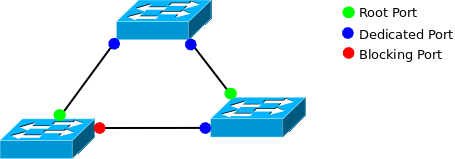
\includegraphics[width=0.7\textwidth]{port_states.png}
    \caption{An example of STP port states}
    \label{fig:port_states}
    %TODO: redo in tikz
\end{figure}

\subsection{STP Packets}
%TODO: rewrite (must include default configuration)
\label{stp_packet}
%TODO: redo in tikz
\begin{figure}[h]
    \centering
    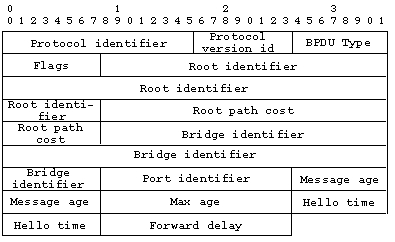
\includegraphics[width=0.8\textwidth]{stp_bpdu.png}
    \caption{An STP BPDU}
    \label{fig:stp_bpdu}
\end{figure}
In this section we will explain the parts of an STP Bridge Protocol Data Unit (BPDU), as seen in Figure~\ref{fig:stp_bpdu}, used in this project.
\begin{itemize}
    \item \textbf{Flags}: The Flags Byte is used for the \textit{Topology Change} and \textit{Topology Change Acknowledgement} flags.
    \item \textbf{Root/Bridge Identifier}: The Identifier consists of three parts and has the same layout for the Root and regular bridges:
        \begin{itemize}
            \item Priority (4 Bits): A value between 0 and 61440 configurable in increments of 4096
            \item System ID Extension (12 Bits): Used for keeping the Bridge ID unique if multiple VLANs are configured for a Bridge
            \item Bridge MAC (6 Byte): The MAC address of the Bridge
        \end{itemize}
        The conjunction of these three parts is used in comparisons as one large 8 Byte number.
    \item \textbf{Root Path Cost}: The Root Path Cost is the sum of all Port Costs (which can be configured in the Bridge) along the current path. The Root Path Cost in packets sent by the Root is 0.
    \item \textbf{Message Age}: The Message Age is the number of Bridges that have been passed (in addition to the Root) along the current path.
    \item \textbf{Forward Delay}: After this time, if no superior packet was received, a Root, or Blocking Port will transition to Dedicated.
        Note that if a Root Port transitions to Dedicated state that means the Bridge now assumes it is the Root.
\end{itemize}
A BPDU only contains information about the root and the bridge that sent the package.
This means that if there is a bridge between these two, we will not know about its id.
We will however still know that it is there, because of the message age.
During the buildup of the tree it is possible to obtain information on intermediate nodes.
This possibility is explained more in-depth in the section on packet handling (Section~\ref{packet_handling}).

\subsection{Spanning Tree Algorithm}
%TODO: fix algorithm placement and explain constraints required by original paper, and how this fulfills them
STP enabled Bridges run through Algorithm~\ref{alg:stp} when receiving an STP packet.
It ensures that information on the global Root is kept up to date and that Ports that receive a superior STP BPDU are disabled.

\begin{algorithm}[h]
    \DontPrintSemicolon
    \KwData{\\
    $received$ = received packet\;
    $current$ = data of the current Bridge\;
    }
    \;
    \If{$received.rootId < current.rootId$}{
        \tcc{There is a new Root in the network}
        $current.rootId=other.rootId$\;
        set receiving port as Root-Port\;
        set other ports to Dedicated\;
    }{
        \uIf{$received.rootPathCost<current.rootPathCost$}{
            \tcc{This means that the path via the other Bridge is shorter, so this should be our new Root-Path}
            set receiving port as Root-Port\;
            set other ports to Dedicated\;
        }
        \ElseIf{$received.rootPathCost==current.rootPathCost \land received.bridgeId<current.bridgeId$}{
            \tcc{Both Bridges are equidistant from the Root, but the other Bridge has a lower Bridge Identifier and should be the Dedicated Bridge on the connection}
            set receiving port as Blocking Port\;
        }
        \tcc{Finally check if the transitions described in section \ref{stp_packet} on \textbf{STP Packets} is necessary}
        doPacketTimeOutTransitions()\;
    }
    
    \caption{Spanning Tree Bridge Algorithm}
    \label{alg:stp}
\end{algorithm}

\section{Technologies used}
\subsection{PCAP}
\label{pcap}
PCAP is a shortening of packet capture.
It used to be a part of the \textit{tcpdump} tool before it was pulled into it's own library.
We used the UNIX version \textit{libpcap} for this project.
\textit{Libpcap} is a C library and can be directly linked with C and C++ without using a wrapper.
It provides functions for opening live network devices and \textit{.pcapng} files.
After starting a live capture on a device, \textit{libpcap} will call a callback function for every packet received on the opened interface.
The prototype of the callback function looks as follows:
\begin{lstlisting}[caption=Pcap Callback Prototype]
typedef void (*pcap_handler)(u_char *user, 
const struct pcap_pkthdr *h,
const u_char *bytes);
\end{lstlisting}
Where the parameters are:
\begin{itemize}
    \item \textbf{u\_char *user}: This parameter is used to pass user defined parameters.
    \item \textbf{pcap\_pkthdr *h}: The header contains useful information about the packet, like source and destination addresses and size.
    \item \textbf{u\_char *bytes}: This array contains the actual (binary) data of the packet.
\end{itemize}
The \textbf{typedef void} (*pcap\_handler) part of the prototype just means that the function returns a \textbf{void *}.

Usage of this function will be covered more in-depth in the chapter on the tool itself (Chapter~\ref{stp_gen}).
\subsection{JSON}
\label{json}
JSON stands for Java Script Object Notation and was used for two reasons:
\begin{enumerate}
    \item It keeps the network communication independent from any and all programming languages used.
    \item Utility libraries for JSON are easily available for most programming and scripting languages, saving us the work of inventing and implementing our own notation.
\end{enumerate}
JSON has a simple notation for declaring objects and arrays, as well as primitive data types.
An example is shown in Listing~\ref{lst:json}.
\lstinputlisting[caption=JSON example, label=lst:json]{../listings/json/example.json}
The JSON library used in this project is \textit{jsoncpp}\cite{jsoncpp}.

\subsection{TikZ}
We chose TikZ ist kein Zeichenprogramm (TikZ) as the file format for our output.
This choice fell to it because it would be very easy to create TikZ code programatically.
It is also easy to modify after creation and very easy to include in a \LaTeX\ paper.
While TikZ is very powerful and therefore complex, the parts we use are fairly simple.
Listing~\ref{lst:tikz_example} shows the TikZ code for Figure~\ref{fig:bc_storm_b}.
\lstinputlisting[caption=A TikZ example, label=lst:tikz_example]{../listings/tikzExample.tex} %TODO: check positioning
